\documentclass[12pt,letterpaper]{article}  
%-------INSTALACIÓN DE PAQUETES-------
% Paquetes de generalidades
%%%%%%%%%%%%%%%%%%%%%%%%%%%%%%%

% Para escribir tildes y eñes
\usepackage[utf8]{inputenc}   

% Para que los títulos de figuras, tablas y otros estén en español
\usepackage[spanish,es-noquoting]{babel} 
	% Cambiar nombre a tablas
	\addto\captionsspanish{\renewcommand{\tablename}{Tabla}}	
    % Cambiar nombre a lista de tablas		
	\addto\captionsspanish{\renewcommand{\listtablename}{Índice de tablas}}	
    % Cambiar nombre a capítulos
	\addto\captionsspanish{\renewcommand{\chaptername}{Sección}}

% Para que la bibligrafía esté en español

\decimalpoint
\usepackage[spanish,es-tabla]{babel}

\usepackage[backend=bibtex]{biblatex}
\addbibresource{referencias.bib}


% Tamaño del área de escritura de la página	
\usepackage{geometry}                         
	\geometry{left=18mm,right=18mm,top=23mm,bottom=23mm} 	

% Paquetes para matemática
%%%%%%%%%%%%%%%%%%%%%%%%%%%%%%%

% Los paquetes ams son desarrollados por la American Mathematical Society y mejoran la escritura de fórmulas y símbolos matemáticos.
\usepackage{amsmath}       
\usepackage{amsfonts}     	
\usepackage{amssymb}

% Paquetes para manejo de gráficas y figuras
%%%%%%%%%%%%%%%%%%%%%%%%%%%%%%%

% Para insertar gráficas
\usepackage{graphicx}     	

% Para colocar varias subfiguras
\usepackage[lofdepth,lotdepth]{subfig}

% Para crear gráficos vectoriales con un lenguaje descriptivo/geométrico
\usepackage{tikz}

% Para crear circuitos vectoriales basados en TikZ
\usepackage[american]{circuitikz}

% Paquetes relacionados con el estilo 
%%%%%%%%%%%%%%%%%%%%%%%%%%%%%%%

% Para la presentación correcta de magnitudes y unidades
\usepackage{siunitx}	

% Para hipervínculos y marcadores
\usepackage[colorlinks=true,urlcolor=blue,linkcolor=blue,citecolor=green]{hyperref}
	\urlstyle{same}

% Para ubicar las tablas y figuras justo después del texto
\usepackage{float}	

% Para hacer tablas más estilizadas
\usepackage{booktabs}		

% Para hacer secciones con múltiples columnas
\usepackage{multicol}

% Para insertar código fuente estilizado
\usepackage{listings}
	\lstset{basicstyle=\ttfamily,breaklines=true}
    \lstset{numbers=left, numberstyle=\tiny, stepnumber=1, numbersep=6pt}

% Para agregar código con formato de Matlab
%\usepackage[numbered,autolinebreaks]{mcode}

% Para utilizar el número de páginas
\usepackage{lastpage}

% Para manejar los encabezados y pies de página
\usepackage{fancyhdr}
	% Contenido de los encabezados y pies de pagina
	\pagestyle{fancy}

% Misceláneos
%%%%%%%%%%%%%%%%%%%%%%%%%%%%%%%

% Para insertar símbolos extraños
\usepackage{marvosym}

%%libreria tikz

\usepackage{tikz}
\usetikzlibrary{shapes.geometric, arrows}

%% acento periodico

\usepackage{yhmath}

%% quitar enumeracion en ecuaciones

\usepackage{amsmath}
%----------Encabezado---------
\lhead{Matemática}
	\chead{}
	\rhead{}
	%\lfoot{Facultad de Ingeniería}
	\cfoot{\thepage\ de \pageref{LastPage}}
	%\rfoot{Universidad Nacional de Mar del Plata}

% Comandos especiales
\newcommand{\EIE}{\textsc{Facultad \Lightning~ Ingeniería}}
%---------------INICIO DE DOCUMENTO--------------
\begin{document}
% portada
\begin{titlepage}
                




\centering
\hspace{10pt}

\begin{figure}[h]
\centering
\fbox{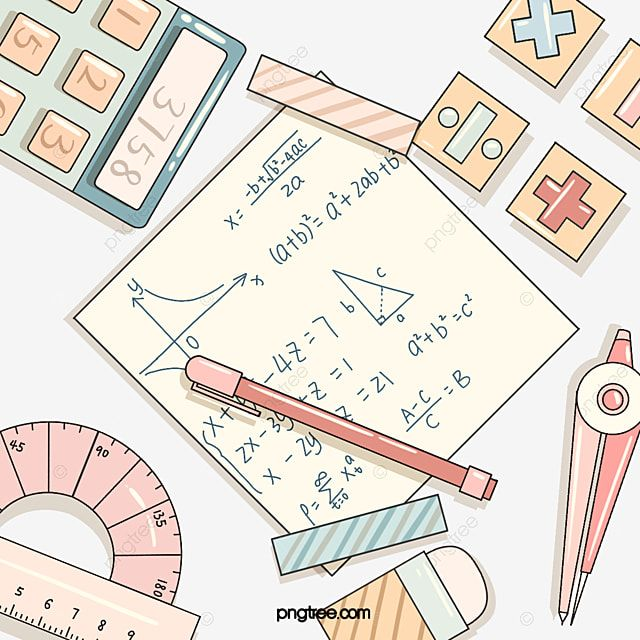
\includegraphics[width=0.8\linewidth]{images/math.jpg}}
\label{1.0}
\end{figure}


{\scshape\Huge  \par}
{\scshape\Huge Matemática \par}
\vspace{1cm}

{\Large Autor: \par}
{\Large Vazquez, Leonardo David \par}
\vspace{1cm}

{\Large Contacto: \par}
{\Large vazquezleonardodavid@outlook.com \par}
\vspace{1cm}

\end{titlepage}
%\maketitle
%\thispagestyle{empty} 
%\maketitle
% índice
{
  \hypersetup{linkcolor=black}
  \tableofcontents
}
\bigskip

%-----------INICIO------------
\newpage
\section{Números naturales}
Los números naturales son aquellos números exactos y positivos: 1, 2, 3, 4, 5... Y así sucesivamente. \\ Hay varias propiedades para una de las operaciones básicas (suma, resta, multiplicación y división):
\begin{itemize}
\item Propiedad conmutativa (suma): \vskip \centering $5 + 8 = 13$
                             \vskip \centering $8 + 5 = 13$ \vskip
\raggedright 
\item Propiedad conmutativa (multiplicación): \vskip \centering $2\cdot3 =6$
                             \vskip \centering $3\cdot2= 6$
\vskip
\raggedright 
\item Propiedad asociativa (suma): \vskip \centering $1 +(4+7) = 1+11=12$
                             \vskip \centering $(1+4) + 7 =5+7= 12$ \vskip
\raggedright 
\item Propiedad asociativa (multiplicación): \vskip \centering $2\cdot(3\cdot5)=2\cdot15=30$
                             \vskip \centering $(2\cdot3)\cdot5=6\cdot5=30$
\vskip
\raggedright 
\item Propiedad distributiva (suma): \vskip \centering $2\cdot(3+5)=2\cdot8=16$
                             \vskip \centering $2\cdot(3+5)=2\cdot3+2\cdot5=6+10=16$ \vskip
\raggedright 
\item Propiedad distributiva (resta): \vskip \centering $3\cdot(8-3)=3\cdot5=15$
                             \vskip \centering $3\cdot(8-3)=3\cdot8-3\cdot3=24-9=15$

\end{itemize}
\textit{No te olvides de separar en términos:} Separar en términos nos sirve para saber qué cuenta hacer primero sin cometer errores:

\begin{equation}
    \notag
    5\cdot3+4 = \overbrace{5\cdot3} + 4 = 15+4=19 
\end{equation}



\raggedright
Ejercicios:


\begin{enumerate}
\renewcommand{\labelenumi}{{\theenumi})}
\item $10+5-2+1$
\item $15\cdot0+10\cdot3-25/5$
\item $(27+5)\cdot6-8\cdot(4+3\cdot2)$
\end{enumerate}
%-------------------------------
\newpage
\section{Ecuaciones - Parte I}
La manera de resolver una ecuación es despejar. Despejar significa dejar a la incógnita ($x$ o $y$ o cualquier letra) de un lado y pasar todo lo demás para el otro lado.\\
\medskip
Resolvamos esta ecuación:\\
\begin{equation}
    \notag
    2\cdot x + 5 = 13
\end{equation}

 
Acá tenemos que pasar primero el $5$ que está sumando. Lo pasamos para  el otro lado pero le cambiamos el signo:\\
\begin{equation}
    \notag
    2\cdot x = 13 - 5
\end{equation}


Luego tenemos que pasar el $2$ que está multiplicando a la incógnita $x$. Para eso lo pasamos hacia el otro lado dividiendo:\\

\begin{equation}
    \notag
    x = (13 - 5)/2
\end{equation}



De esta forma, resolvemos primero la operación entre paréntesis:\\

\begin{equation}
    \notag
    x = 8/2
\end{equation}


Por lo tanto nuestra incógnita está despejada y vale $x=4$.\\
\medskip
Las reglas básicas para pasar de términos son:

\begin{itemize}
    \item Lo que está sumando pasa restando:
    \begin{equation}
    \notag
       x+2=5 \longrightarrow x=5-2 
    \end{equation}

       
    \item Lo que está restando pasa sumando:
    \begin{equation}
    \notag
    x-3 = 9 \longrightarrow x=9+3 
    \end{equation}
    
    \item Lo que está multiplicando pasa dividiendo: 
    \begin{equation}
    \notag
     3\cdot x =4 \longrightarrow x=4/3 
    \end{equation}
   
    \item Lo que está dividiendo pasa multiplicando: 
    \begin{equation}
    \notag
       x/2=5 \longrightarrow x=5\cdot2 
    \end{equation}
  
\end{itemize}

Ejercicios:

\begin{enumerate}
\renewcommand{\labelenumi}{{\theenumi})}
\item $15=x+4$
\item $27+x=2$
\item $5\cdot x + 1 = 15$
\item $ 52-12 = x-19+20$
\item $2\cdot x +5\cdot ( 25-20) = 7\cdot7 -10$
\item $x\cdot6 -2 = -2$
\item $2\cdot(x+2)=-4$
\item $x+4\cdot(x+3)=0$
\item $3\cdot(2\cdot x+1)+x=5\cdot x$
\end{enumerate}
%-------------------------------
%\newpage
\section{Potencia y Raíz}
Las potencias de un número son operaciones que hacen multiplicar dicho número por sí mismo. Dicho número de multiplicaciones se le llama $Potencia$ o $exponente$. El número a multiplicar se le dice $base$. Veamos un ejemplo:

\begin{equation}
    \notag
    5^2=5\cdot5=25
\end{equation}


El cual es $5$ (base) $al$ $cuadrado$ (exponente $2$). Si elevamos $5$ $a$ $la$ $potencia$ $de$ $3$, es decir $(5^3)$, se le dice $al$ $cubo$. Si elevamos $5$ $a$ $la$ $potencia$ $de$ $4$, el cual es $(5^4)$, se le dice $a$ $la$ $cuarta$ y así sucesivamente.\\
\medskip

Veamos algunas de las propiedades básicas: \\

\begin{itemize}
    \item Potencia neutra: 
    \begin{equation}
        \notag
        a^1=a \longrightarrow 2^1=2
    \end{equation}
    \item Potencia de exponente nulo es una unidad: 
    \begin{equation}
        \notag
        a^0=1 \longrightarrow 2^0=1
    \end{equation} 
    \item Producto de igual base se suman exponentes: 
    \begin{equation}
        \notag
        a^n \cdot a^m = a^{n+m} \longrightarrow 2^2\cdot 2^1=2^3 
    \end{equation} 
    \item Exponente negativa implica división: 
    \begin{equation}
        \notag
        a^{-n}=1/a^n \longrightarrow 2^{-1}=1/2  
    \end{equation} 
    \item División de potencias de igual base es resta de exponentes: 
     \begin{equation}
        \notag
        a^m / a^n = a^{m-n} \longrightarrow 2^3/2^1 = 2^2
    \end{equation} 
    \item Potencia de potencia se multiplican exponentes:
     \begin{equation}
        \notag
        {(a^n)}^m = a^{n\cdot m} \longrightarrow {(2^2)}^2 = 2^4 
    \end{equation}  
    \item Potencia de distintas bases:
     \begin{equation}
        \notag
        (a\cdot b)^n =a^n\cdot b^n \longrightarrow {(2\cdot 3)}^2 = 2^2 \cdot 2^3
    \end{equation}  
    \item Potencia de división:
     \begin{equation}
        \notag
        (a/ b)^n =a^n / b^n \longrightarrow {(2 / 3)}^2 = 2^2 / 2^3
    \end{equation}  
\end{itemize}

¡Son muchas propiedades! Tranquilo/a, puede que no las utilices todas.\\
\medskip

Por otro lado, la Raíz es la operación inversa a la Potencia. La raíz de un número $a$ es un número $b$ que multiplicado tantas veces por sí mismo da el número $a$. Veamos un ejemplo de la raíz cuadrada (El número se denomina índice y el número dentro de la raíz se llama radicando): \\


\begin{equation}
\notag
\sqrt[2]{36}=\sqrt{36}=6 \longrightarrow 6\cdot 6 = 36 
\end{equation} 

Y de la raíz cúbica: \\
\begin{equation}
\notag
\sqrt[3]{125}=5 \longrightarrow 5\cdot 5 \cdot 5 = 125 
\end{equation}


Como era de anticiparse, existe una relación entre la raíz de tal número con la potencia:\\

\begin{equation}
\notag
\sqrt[n]{a^m}=a^{m/n} \longrightarrow \sqrt[3]{2^3}=2^{3/3}=2     
\end{equation}



Veamos algunas de las propiedades básicas: \\

\begin{itemize}
    \item Raíz de producto: 
    \begin{equation}
        \notag
        \sqrt[n]{a\cdot b} = \sqrt[n]{a} \cdot \sqrt[n]{b} \longrightarrow \sqrt{2\cdot 3} = \sqrt{2} \cdot \sqrt{3}
    \end{equation}
    
    \item Raíz de división: 
    \begin{equation}
        \notag
        \sqrt[n]{a: b} = \sqrt[n]{a} : \sqrt[n]{b} \longrightarrow \sqrt{2: 3} = \sqrt{2} : \sqrt{3}
    \end{equation}
    
    \item Como caso especial:
      \begin{equation}
        \notag
         \sqrt[2]{a}\cdot \sqrt[2]{a}=\sqrt[2]{a}^2 = a     
            \end{equation}

\end{itemize}

\medskip
Ejercicios:

\begin{enumerate}
\renewcommand{\labelenumi}{{\theenumi})}
\item $8^2$
\item $3^3$
\item $\sqrt{9}$
\item $\sqrt{100}$

\end{enumerate}
%-------------------------------
%\newpage
\section{Fracciones}
¿Qué es una fracción? Una fracción es una "parte" de un entero. Por ejemplo, si tengo la mitad de un chocolate, esa mitad es una fracción. Las fracciones se expresan de la siguiente manera:\\

\begin{equation}
    \notag
    \frac{3}{4} \longrightarrow \frac{Numerador}{Denominador}
\end{equation}


El Numerador es la cantidad de partes "que tengo" mientras que el Denominador es la cantidad de partes en la cual está partido el entero. En la figura siguiente se ejemplifica visualmente: 

\begin{figure}[H]
\centering
\fbox{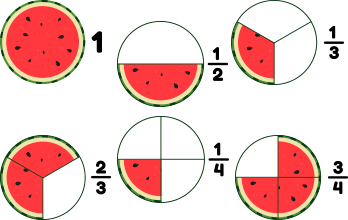
\includegraphics[width=0.5\linewidth]{images/fraccion.png}}
\label{1.0}
\end{figure}

Sin entrar en complicaciones, veamos simplemente las operaciones básicas de las fracciones: \\

\begin{itemize}
    \item Suma o resta con igual denominador: 
    \begin{equation}
        \notag
         \frac{a}{B} + \frac{b}{B} = \frac{a+ b}{B} \longrightarrow \frac{1}{2} + \frac{4}{2} = \frac{5}{2}
    \end{equation}
    \item Suma o resta con distinto denominador:
    \begin{equation}
        \notag
         \frac{a}{b} + \frac{c}{d} = \frac{a\cdot d + c\cdot b}{b\cdot d} \longrightarrow \frac{1}{2} + \frac{1}{3}=\frac{5}{6}
    \end{equation}
    \item Producto de fracciones: 
    \begin{equation}
        \notag
        \frac{a}{b}\cdot \frac{c}{d}=\frac{a\cdot c }{b \cdot d} \longrightarrow \frac{1}{2}\cdot \frac{3}{4}=\frac{3}{8}
    \end{equation}
    \item División de fracciones: 
    \begin{equation}
        \notag
            \frac{a}{b} : \frac{c}{d}=\frac{a\cdot d }{b \cdot c} \longrightarrow \frac{1}{2}\cdot \frac{3}{4}=\frac{4}{6}
    \end{equation}
\end{itemize}

Otra forma de sumar/restar varias fracciones es la siguiente: En el denominador se coloca el producto de denominadores $D=d_1\cdot d_2 \cdot d_3$ y en el numerador $N$ se realiza la suma/resta de los productos entre cada numerador $n_1, n_2, n_3$ y la división entre el denominador $D$ y el denominador $d_1, d_2, d_3$:

\begin{equation}
    \notag
    \frac{n_1}{d_1}\pm\frac{n_2}{d_2}\pm\frac{n_3}{d_3}=\frac{n_1\cdot (D:d_1) \pm n_2\cdot (D:d_2)\pm n_3\cdot (D:d_3) }{D}   
\end{equation}

\medskip
Veamos un ejemplo:
\begin{equation}
     \notag
    \frac{2}{3}+\frac{4}{5}-\frac{6}{7}  
\end{equation}
Calculamos $D = 3\cdot 5 \cdot 7 = 105$, luego:

\begin{equation}
     \notag
    \frac{2}{3}+\frac{4}{5}+\frac{6}{7} =  =\frac{2\cdot (105:3) + 4\cdot (105:5)- 6\cdot (105:7) }{105}
\end{equation}

Resolvemos las divisiones y sumamos y restamos:

\begin{equation}
     \notag
    \frac{2}{3}+\frac{4}{5}+\frac{6}{7} =  =\frac{2\cdot 35 + 4\cdot 21- 6\cdot 15 }{105} = \frac{64}{105}
\end{equation}

Ejercicios:\\

\begin{enumerate}
\renewcommand{\labelenumi}{{\theenumi})}
\item $\frac{9}{3}-\frac{5}{6}$
\item $\frac{2}{5}\cdot \frac{12}{1}$
\item $\frac{4}{5}\cdot \frac{6}{1} : \frac{2}{11}$

\end{enumerate}

%-------------------------------
%\newpage
\section{Números decimales}
Una expresión decimal es un número cuya parte "no entera" se expresa mediante el uso de la coma:\\
\begin{equation}
    \notag
    1,489
\end{equation}

Existen 3 tipos de números decimales:

\begin{itemize}
    \item Decimales finitos: $ 2,53$
    \item Periódicos puros:  $1,\wideparen{43}=1,43434343...$
    \item Periódicos Mixtos: $ 0,42\widepared{16}=0,42161616...$ 
    
\end{itemize}

Veamos la forma de escribir un número decimal como una fracción.. \\
\medskip

\begin{itemize}
    \item Caso 1: Decimales no periódicos. Se escribe el número completo sin coma en el numerador y luego en el denominador un $1$ seguido de tantos ceros como decimales hayan:
     \begin{equation}
    \notag
      5,47 = \frac{547}{100}
     \end{equation}
      
      
    \item Caso 2: Decimales periódicos puros. En el numerador se resta el número completo sin coma menos la parte entera. En el denominador se escriben tantos 9 como decimales hayan.
     \begin{equation}
    \notag
    5,\wideparen{47} = \frac{547-5}{99}=\frac{542}{99}
     \end{equation}
     
     
    \item Caso 3: Caso 3: Decimales periódicos Mixtos. En el numerador se resta el número completo sin coma menos los números que no se repiten sin coma. En el denominador se escriben tantos 9 como decimales periódicos hayan seguido de tantos 0 como decimales no periódicos hayan.
    \begin{equation}
    \notag
    5,62\wideparen{7} = \frac{5627-562}{900} = \frac{5065}{900}
     \end{equation}
\end{itemize}\\

Ejercicios: Expresar como fracción\\

\begin{enumerate}
\renewcommand{\labelenumi}{{\theenumi})}
\item $0,04$
\item $0,\wideparen{44}$
\item $99,9\wideparen{999}$
\end{enumerate}

%-------------------------------
%\newpage
\section{Simplificación y Racionalización}
Simplificar implica lograr que una expresión matemática esté compuesta por un único término lo más sencillo posible. Veamos un ejemplo:

\begin{equation}
    \notag
    \frac{0.\wideparen{2}+1,1\wideparen{1}}{0,\wideparen{6}} -1 =?
\end{equation}

Desde el capitulo anterior, sabemos que a los números decimales podemos expresarlos como números fraccionarios:

\begin{equation}
    \notag
    \frac{\frac{2}{9}+\frac{100}{90}}{\frac{6}{9}}-1 =?
\end{equation}

Lo próximo a realizar es una suma de fracciones con distinto denominador: 

\begin{equation}
    \notag
    \frac{\frac{4}{3}}{\frac{6}{9}}-1 = ?
\end{equation}

División de fracciones y luego una simple resta:

\begin{equation}
    \notag
    2-1 = 1
\end{equation}

A pesar de que el proceso sea largo, lo importante aquí a resaltar es la aplicación de los conceptos y propiedades vistas anteriormente.

Por otro lado, racionalizar implica modificar una expresión fraccionaria con raíz en el denominador a una expresión fraccionaria sin raíz en el denominador. El truco es bastante sencillo: Hay que observar el índice de la raíz y la potencia del radicando:

\begin{equation}
    \notag
    \frac{1}{\sqrt[n]{a^b}}
\end{equation}

Luego se multiplica por un entero cuyas raíces en numerador y denominador son iguales y posee igual índice pero distinta potencia al que se desea extraer o racionalizar:

\begin{equation}
    \notag
    \frac{1}{\sqrt[n]{a^b}}\cdot \frac{\sqrt[n]{a^{n-b}}}{\sqrt[n]{a^{n-b}}}
\end{equation}

Haciendo uso de alguna de las propiedades de la potencia y raíz:


\begin{equation}
    \notag
   \sqrt[n]{a^{n-b}} = a^{(n-b)/n}
\end{equation}

\begin{equation}
    \notag
   \sqrt[n]{a^b} = a^{b/n}
\end{equation}

De esta forma: 

\begin{equation}
    \notag
    \frac{1\cdot \sqrt[n]{a^{n-b}} }{a^{b/n} \cdot  a^{(n-b)/n}} 
\end{equation}

Pero exponentes de potencias con igual base se suman por lo que:

\begin{equation}
    \notag
   a^{b/n} \cdot  a^{(n-b)/n}= a 
\end{equation}

Por lo que la formula para racionalizar es simplemente: 

\begin{equation}
    \notag
    \frac{1}{\sqrt[n]{a^b}} = \frac{\sqrt[n]{a^{n-b}}}{a}
\end{equation}

Veamos un ejemplo sencillo:


\begin{equation}
    \notag
    \frac{4}{\sqrt[5]{7^3}} 
\end{equation}

En este caso solo basta con mirar nuestra formula y darse cuenta que: $n=5$, $a=7$ y $b=3$ por lo que $n-b=2$. De esta forma:

\begin{equation}
    \notag
    \frac{4}{\sqrt[5]{7^3}} = \frac{4\cdot \sqrt[5]{7^{2}}}{7}
\end{equation}

En muchos casos, puede que te encuentres con expresiones del tipo:

\begin{equation}
    \notag
    \frac{1}{\sqrt{a}+\sqrt{b}}
\end{equation}

La manera de racionalizar esto es multiplicando por un entero que posea en el numerador y denominador el conjugado del denominador de la expresión anterior, es decir, cambiar el signo:

\begin{equation}
    \notag
    \frac{1}{\sqrt{a}+\sqrt{b}}\cdot \frac{\sqrt{a}-\sqrt{b}}{\sqrt{a}-\sqrt{b}}
\end{equation}

Realizando la multiplicación entre denominadores se obtiene fácilmente:

\begin{equation}
    \notag
     \frac{1}{\sqrt{a}+\sqrt{b}}= \frac{\sqrt{a}-\sqrt{b}}{a-b}
\end{equation}
$Observación$: En caso de que en el denominador no sean ambos términos con raíz necesariamente, el procedimiento consiste en multiplicar por un entero conjugado.\\
\medskip
Veamos un ejemplo sencillo: 

\begin{equation}
    \notag
    \frac{1}{\sqrt{2}+\sqrt{3}} 
\end{equation}
Multiplicamos por el entero conjugado:

\begin{equation}
    \notag
    =\frac{1}{(\sqrt{2}+\sqrt{3})} \cdot \frac{\sqrt{2}-\sqrt{3}}{(\sqrt{2}-\sqrt{3})}
\end{equation}

\begin{equation}
    \notag
=\frac{\sqrt{2}-\sqrt{3}}{(\sqrt{2}\cdot \sqrt{2})-(\sqrt{3}\cdot \sqrt{2})+(\sqrt{3}\cdot \sqrt{2})-(\sqrt{3}\cdot \sqrt{3})}
\end{equation}

Finalmente:
\begin{equation}
    \notag
    \frac{1}{\sqrt{2}+\sqrt{3}} = \frac{\sqrt{2}-\sqrt{3}}{2-3} =  \frac{\sqrt{2}-\sqrt{3}}{-1} 
\end{equation}

Ejercicios: Simplificar

\begin{enumerate}
\renewcommand{\labelenumi}{{\theenumi})}
\item $7\cdot \sqrt[3]{9}- \frac{1}{3}\cdot  \sqrt[3]{9}$
\item $\frac{3}{5}\cdot \sqrt{7}-\frac{3}{4}$
\item $3\cdot \sqrt[3]{64}-\sqrt[3]{27}$
\item $\sqrt{80}\cdot \sqrt{30}$
\end{enumerate}

Ejercicios: Resolver

\begin{enumerate}
\renewcommand{\labelenumi}{{\theenumi})}
\item $(0,1)^{-1}+\frac{1}{2}:\frac{-3}{2}-\sqrt{1/4}$
\item $0,3\cdot \frac{-1}{2}-(2/5)^{-2}$
\item $(\frac{3}{2}-\frac{5}{3})^{-1}+\sqrt{0,\wideparen{1}}$
\end{enumerate}

Ejercicios: Racionalizar

\begin{enumerate}
\renewcommand{\labelenumi}{{\theenumi})}
\item ${13}:(20-\sqrt{15})$
\item $-17:\sqrt{15}$
\item $8:\sqrt[10]{2^4}$
\end{enumerate}
%-------------------------------
%\newpage
\section{Ecuaciones - Parte II}
Dado que hemos visto hasta aquí una amplia variedad de propiedades, intentemos resolver brevemente una ecuación un tanto difícil: 

\begin{equation}
    \notag
    \frac{2-3\cdot x}{4} = (-1+4)
\end{equation}

Resolvemos la resta de la derecha y luego lo que esta dividiendo a la izquierda pasa multiplicando hacia la derecha:

\begin{equation}
    \notag
    2-3\cdot x = 3\cdot 4 
\end{equation}

\begin{equation}
    \notag
    2-3\cdot x = 12
\end{equation}

El $2$ que suma pasa restando:

\begin{equation}
    \notag
    -3\cdot x = 12-2
\end{equation}

\begin{equation}
    \notag
    -3\cdot x = 10
\end{equation}

Finalmente pasamos dividiendo el $-3$:

\begin{equation}
    \notag
    x = \frac{-10}{3}
\end{equation}


Veamos otro ejemplo más difícil:

\begin{equation}
    \notag
    (x+5)^2=4
\end{equation}

La potencia la pasamos como raíz cuadrada:

\begin{equation}
    \notag
    x+5 = \sqrt{4} 
\end{equation}

La raíz cuadrada de 4 es 2, de esta forma despejamos fácilmente la incógnita:

\begin{equation}
    \notag
    x = 2-5 = -3 
\end{equation}

Ejercicios: Despejar $x$
\begin{enumerate}
\renewcommand{\labelenumi}{{\theenumi})}
\item $1/4 \cdot x -1/2\cdot 3/5 =2/3$
\item $(3/2 \cdot x -5)^2 = 4/9$
\item $3/2\cdot (x-3)+0,5 = 4/5 -1/3 \cdot x$
\end{enumerate}

%-------------------------------
%\newpage
\section{Sistemas de ecuaciones}
Un sistema de ecuaciones de dos incógnitas consiste en dos ecuaciones. Lo que debemos hacer es despejar una de ellas en función de la otra de una de las dos ecuaciones. Luego, expresar en la segunda ecuación en función de una sola incógnita para luego hallar la segunda. ¡Qué trabalenguas! \\

Veamos un ejemplo:

\begin{equation}
    \notag
     \left\{ \begin{array}{lcc}
             x + y =3 
             \\2\cdot x + y = 4
             \end{array}
   \right.
\end{equation}

De la primer ecuación vamos a despejar $x$:

\begin{equation}
    \notag
    x = 3 - y
\end{equation}

Luego, vamos a la segunda ecuación y donde esté $x$ colocamos$(3+y)$

\begin{equation}
    \notag
    2\cdot  ( 3 - y ) +y =4
\end{equation}

Una vez que tenemos la ecuación de una sola incógnita, despejamos la $y$:

\begin{equation}
    \notag
    -\cdot y = 4- 6 =-2
\end{equation}

Por lo tanto $y=2$ y $x=1$.\\
\medskip

Ejercicios: Encontrar $x$ e $y$
\begin{enumerate}
\renewcommand{\labelenumi}{{\theenumi})}
\item 
    \begin{equation}
    \notag
     \left\{ \begin{array}{lcc}
             4\cdot x +y =-5 
             \\2\cdot x + y = 4
             \end{array}
   \right.
   \end{equation}
\item 
    \begin{equation}
    \notag
     \left\{ \begin{array}{lcc}
             -5\cdot x +2\cdot y =2
             \\3\cdot x-4\cdot  y = 5
             \end{array}
   \right.
     \end{equation}


\end{enumerate}


%-------------------------------
%-------------------------------
\newpage
\section*{Examen Integrador}
\begin{enumerate}
\renewcommand{\labelenumi}{{\theenumi})}
\item Simplificar:
 \begin{enumerate}
    \item $5\sqrt{63}+3\sqrt{28}$
    \item $\frac{3}{2}\sqrt{11}-5\cdot \sqrt{11}$
   \end{enumerate}
\item Resolver:
    \begin{enumerate}
        \item $(\frac{8}{2})^{-1}+\frac{2}{3}:\frac{-1}{2}+\sqrt{\frac{9}{4}}-\frac{9}{2}$
        \item $\frac{2}{3}+\frac{1}{3}\cdot (\frac{2}{3}+0,\wideparen{2})-0,1$
     \end{enumerate}
\item Calcular:
    \begin{equation}
        \notag
        -\frac{3}{4}\cdot (x-2) +\frac{3}{2}=\frac{7}{3}+\frac{1}{2}\cdot x
    \end{equation}
\item Encontrar $x$ e $y$ tanto analitíticamente como gráficamente:
    \begin{equation}
    \notag
        \left\{ \begin{array}{lcc}
                 3\cdot x + y = 0,75
                 \\0,5\cdot x-2\cdot  y = 4
                 \end{array}
        \right.
    \end{equation}
\end{enumerate}

%-------------------------------

      

\bigskip

\end{document}
